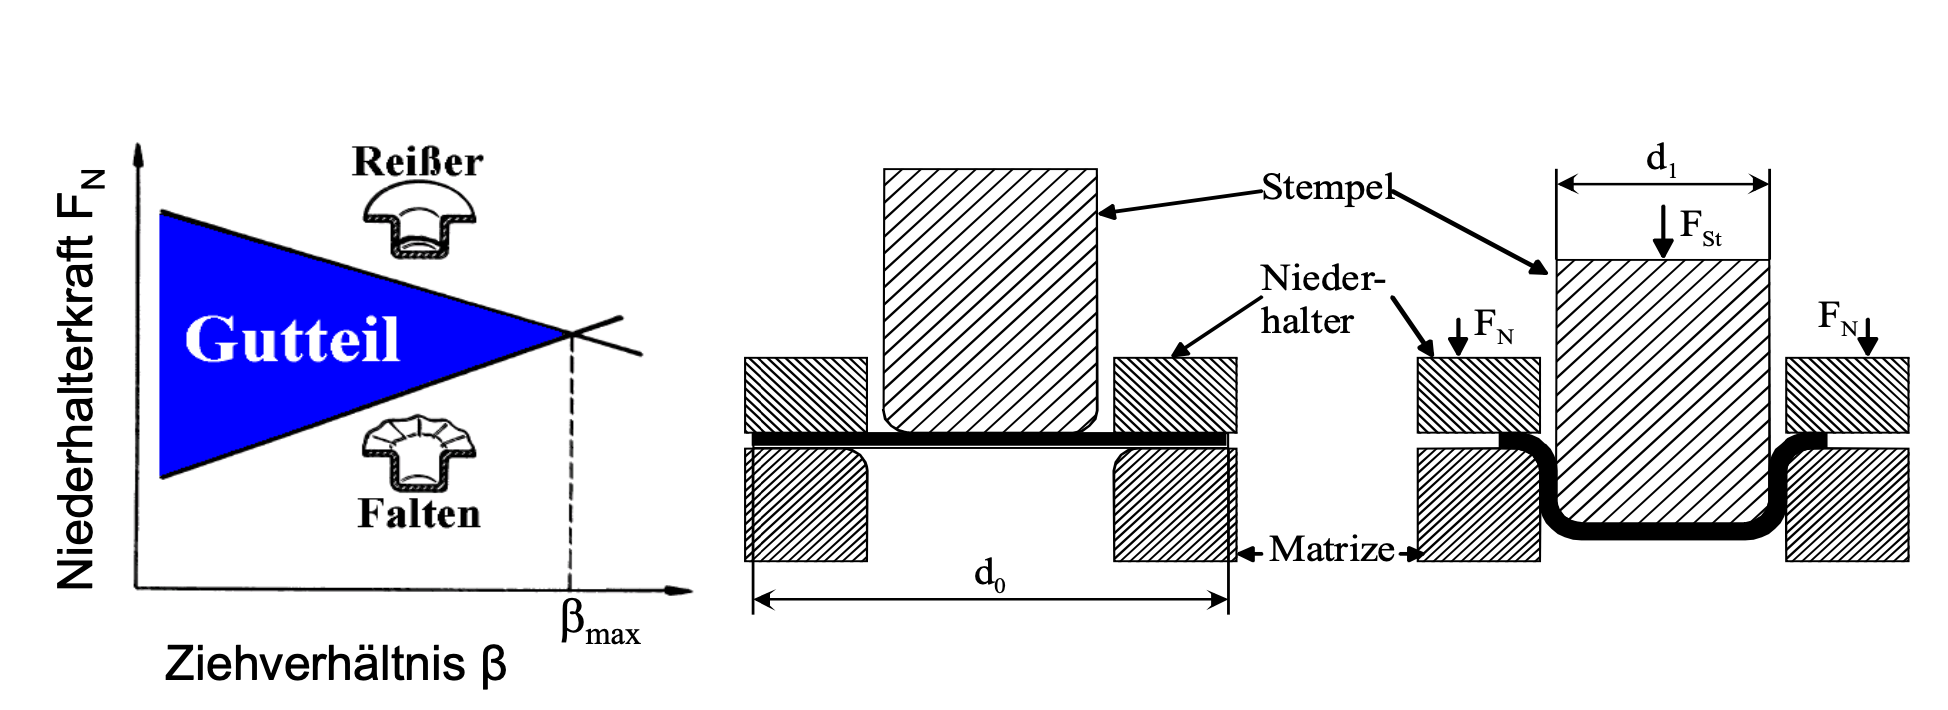
\includegraphics[width = 70mm]{src/images/Tiefziehen.png}




\begin{minipage}{0.5\linewidth}
    \[
    \boxed{     
        \begin{aligned}
            \beta &=\frac{d_0}{d_1} = \frac{d_{n - 1}}{d_n}\\
            \beta_{ges} &= \beta_1 \cdot \beta_2 ... \leq  6.5\\
            \beta_1 &\leq 2\\
            \beta_2 &\leq 1.6
        \end{aligned}
        }
    \]
\end{minipage}
\begin{minipage}{0.5\linewidth}
    \item $\beta$: Ziehverhältnis
    \item $d_0$: Durchmesser vor dem Ziehen
    \item $d_1$: Durchmesser nach dem Ziehen
    \item $\beta_{ges}$: Gesamtziehverhältnis
\end{minipage}
\vspace{1mm}
